\documentclass{article}
\usepackage[paperwidth=30cm,paperheight=20cm,margin=0.2cm]{geometry}
\usepackage{tikz}
\usepackage{xcolor}
\usepackage{amsmath}
\usepackage{amssymb}
\usetikzlibrary{arrows.meta, positioning, fit, backgrounds, calc}
\pagestyle{empty}
\definecolor{headerfg}{HTML}{2C3E50}
\definecolor{iobg}{HTML}{ffccdd}
\definecolor{ioborder}{HTML}{ff80aa}
\definecolor{ocrbg}{HTML}{FBF0CC}
\definecolor{ocrborder}{HTML}{C8A030}
\definecolor{entbg}{HTML}{DAEAF6}
\definecolor{entborder}{HTML}{4A86C8}
\definecolor{attbg}{HTML}{D8EDCF}
\definecolor{attborder}{HTML}{5A9E5A}
\definecolor{valbg}{HTML}{FDE8D0}
\definecolor{valueborder}{HTML}{E8945A}
\definecolor{filterbg}{HTML}{E4D5EF}
\definecolor{filterborder}{HTML}{8E5FAD}
\definecolor{codebg}{HTML}{F0F2F5}
\definecolor{codeborder}{HTML}{BCC4CE}
\definecolor{arrowcol}{HTML}{34495E}
\definecolor{secborder}{HTML}{A0A0A0}
\tikzset{
    mainbox/.style 2 args={rectangle, rounded corners=3pt, fill=#1, draw=#2, line width=1.8pt, text width=4.2cm, align=left, inner sep=5pt, font=\footnotesize, text=headerfg},
    iobox/.style 2 args={rectangle, rounded corners=3pt, fill=#1, draw=#2, line width=1.8pt, text width=3.7cm, align=left, inner sep=5pt, font=\footnotesize, text=headerfg},
    narrowmainbox/.style 2 args={rectangle, rounded corners=3pt, fill=#1, draw=#2, line width=1.8pt, text width=5.0cm, align=left, inner sep=5pt, font=\footnotesize, text=headerfg},
    widemainbox/.style 2 args={rectangle, rounded corners=3pt, fill=#1, draw=#2, line width=1.8pt, text width=6.0cm, align=left, inner sep=5pt, font=\footnotesize, text=headerfg},
    codeblock/.style={rectangle, rounded corners=2pt, draw=codeborder, fill=codebg, line width=1.0pt, inner sep=4pt, font=\ttfamily\scriptsize, align=left, text=headerfg, text width=4.0cm},
    myarrow/.style={-{Stealth[length=6pt, width=4.5pt]}, arrowcol, line width=1.1pt},
    sectionbg/.style={rectangle, rounded corners=6pt, fill=none, draw=secborder, dashed, line width=1.2pt, inner sep=10pt},
    sectionlabel/.style={font=\bfseries, text=headerfg!60},
    secarrow/.style={-{Stealth[length=8pt, width=6pt]}, arrowcol!40, line width=1.4pt},
}
\begin{document}
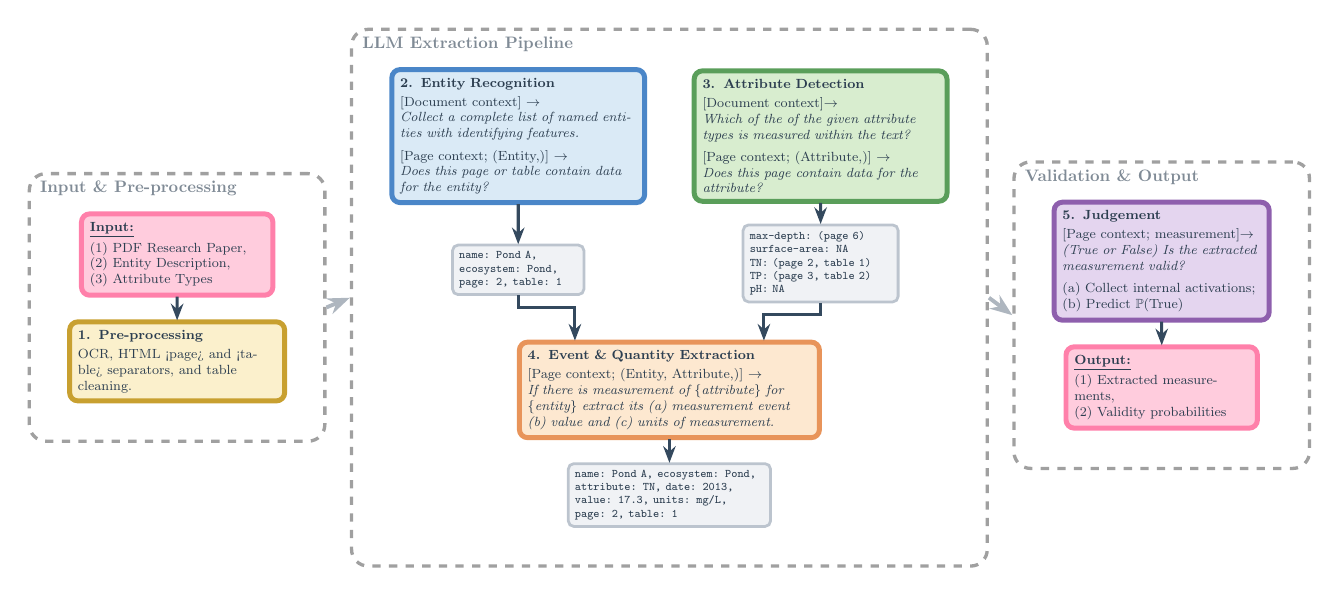
\begin{tikzpicture}[node distance=0.45cm, scale=0.60, transform shape]
\node[narrowmainbox={entbg}{entborder}] (e1box) at (-3.2, 0)
    {\textbf{2.\enspace Entity Recognition}\\[2pt] [Document context] $\rightarrow$ \\ \emph{Collect a complete list of named entities with identifying features.} \\ \vspace{4pt} [Page context; (Entity,)] $\rightarrow$ \\ \emph{Does this page or table contain data for the entity?}};
\node[codeblock, text width=2.5cm, below=0.85cm of e1box] (e1code) {name: Pond A, \\ ecosystem: Pond,\\ page: 2, table: 1\\};
\draw[myarrow] (e1box.south) -- (e1code.north);
\node[narrowmainbox={attbg}{attborder}] (a1box) at (3.2, 0)
    {\textbf{3.\enspace Attribute Detection}\\[2pt] [Document context]$\rightarrow$\\ \emph{Which of the of the given attribute types is measured within the text?}\\ \vspace{4pt} [Page context; (Attribute,)] $\rightarrow$ \\ \emph{Does this page contain data for the attribute?}};
\node[codeblock, text width=3.0cm, below=0.45cm of a1box] (a1code) {max-depth: (page 6)\\ surface-area: NA\\ TN: (page 2, table 1)\\ TP: (page 3, table 2)\\ pH: NA};
\draw[myarrow] (a1box.south) -- (a1code.north);
\path let \p1=(e1code.south), \p2=(a1code.south) in coordinate (val_top) at (0, {min(\y1,\y2) - 0.8cm});
\node[widemainbox={valbg}{valueborder}, anchor=north] (valuebox) at (val_top)
    {\textbf{4.\enspace Event \& Quantity Extraction}\\[2pt] [Page context; (Entity, Attribute,)] $\rightarrow$\\ \emph{If there is measurement of \{attribute\} for \{entity\} extract its (a) measurement event (b) value and (c) units of measurement.}};
\draw[myarrow] (e1code.south) -- ++(0,-0.25) -| ([xshift=-2.0cm]valuebox.north);
\draw[myarrow] (a1code.south) -- ++(0,-0.25) -| ([xshift=+2.0cm]valuebox.north);
\node[codeblock, text width=4.0cm, below=0.5cm of valuebox] (cleancode) {name: Pond A, ecosystem: Pond,\\ attribute: TN, date: 2013,\\ value: 17.3, units: mg/L,\\ page: 2, table: 1\\};
\draw[myarrow] (valuebox.south) -- (cleancode.north);
\begin{scope}[on background layer]
    \node[sectionbg, fit=(e1box)(e1code)(a1box)(a1code)(valuebox)(cleancode), inner sep=14pt] (sec2) {};
    \node[sectionlabel, anchor=north west] at ([xshift=4pt, yshift=-2pt]sec2.north west) {LLM Extraction Pipeline};
\end{scope}
\path let \p1=(sec2.west) in coordinate (sec1centre) at ({\x1 - 24pt - 80pt}, \y1);
\node[iobox={iobg}{ioborder}] (input) at ([yshift=26pt]sec1centre)
    {\textbf{\underline{Input:}} \\ \vspace{3pt} (1) PDF Research Paper, \\(2) Entity Description, \\(3) Attribute Types};
\node[mainbox={ocrbg}{ocrborder}, below=0.5cm of input] (ocrbox)
    {\textbf{1.\enspace Pre-processing}\\[2pt] OCR, HTML <page> and <table> separators, and table cleaning.};
\draw[myarrow] (input.south) -- (ocrbox.north);
\begin{scope}[on background layer]
    \node[sectionbg, fit=(input)(ocrbox), inner sep=14pt] (sec1) {};
    \node[sectionlabel, anchor=north west] at ([xshift=4pt, yshift=-2pt]sec1.north west) {Input \& Pre-processing};
\end{scope}
\path let \p1=(sec2.east) in coordinate (sec3centre) at ({\x1 + 24pt + 80pt}, \y1);
\node[mainbox={filterbg}{filterborder}] (filterbox) at ([yshift=22pt]sec3centre)
    {\textbf{5.\enspace Judgement}\\[2pt] [Page context; measurement]$\rightarrow$\\ \emph{(True or False) Is the extracted measurement valid?}\\ \vspace{4pt} (a) Collect internal activations;\\ (b) Predict $\mathbb{P}(\text{True})$};
\node[iobox={iobg}{ioborder}, below=0.5cm of filterbox] (output)
    {\textbf{\underline{Output:}} \\ \vspace{3pt} (1) Extracted measurements,\\ (2) Validity probabilities};
\draw[myarrow] (filterbox.south) -- (output.north);
\begin{scope}[on background layer]
    \node[sectionbg, fit=(filterbox)(output), inner sep=14pt] (sec3) {};
    \node[sectionlabel, anchor=north west] at ([xshift=4pt, yshift=-2pt]sec3.north west) {Validation \& Output};
\end{scope}
\draw[secarrow] (sec1.east) -- (sec2.west);
\draw[secarrow] (sec2.east) -- (sec3.west);
\end{tikzpicture}
\end{document}
